% ============================================================================
%  Chapter 6 — Security--Utility Trade-off and Residual Risk
%  Thesis: Generative AI, Privacy & Personal Data — TADJ Mohamed Walid, ESI SBA
%
%  DUAL-MODE FILE (standalone OR \input via \ThesisMaster). \cite{...-TODO}
%  placeholders; unified .bib is separate scaffolding (PHASE5_PLAN.md §4.2).
%
%  CANONICAL BASELINE = final_metrics.json C00000 for all ASR (PHASE5_PLAN.md §4),
%  consistent with Ch4/Ch5. NUMBER SOURCES: ASR/knee -> final_metrics.json;
%  utility -> results/phase3/utility/utility_results.json (faithfulness,
%  context-precision, latency ONLY); L3 firing -> l3_firing.json; per-profile ->
%  final_metrics RQ4_per_profile; SEVERITY (S-gap, Exit 1) ->
%  results/phase3/ablation/metrics/severity_aggregates.json; risk matrix + probes
%  -> committed Phase3_4_Report_Expanded.tex §6/§8 (supervisor-reviewed).
% ============================================================================
\ifdefined\ThesisMaster\else
  \documentclass[11pt,a4paper]{report}
  \usepackage[utf8]{inputenc}
  \usepackage[T1]{fontenc}
  \usepackage{lmodern}
  \usepackage[margin=2.5cm]{geometry}
  \usepackage{booktabs}
  \usepackage{tabularx}
  \usepackage{array}
  \newcolumntype{L}{>{\raggedright\arraybackslash}X}
  \usepackage{amsmath,amssymb}
  \usepackage{graphicx}
  \usepackage{microtype}
  \usepackage{xcolor}
  \usepackage[hidelinks]{hyperref}
  \graphicspath{{../}{../../../phase3/report/}{../../../phase3/tradeoff/}}
  \begin{document}
\fi

\chapter{Security--Utility Trade-off and Residual Risk}
\label{ch:tradeoff}

Chapter~\ref{ch:defenses} established that the full defense stack reduces judged leakage from
$28.8\%$ to $17.3\%$. This chapter asks what that reduction costs, where on the
security--utility frontier a deployment should actually sit, and what risk remains once the
defense is in place. It answers \textbf{RQ5} --- the residual privacy risk after the full
stack, expressed as a quantified leakage score, and its trade-off against utility --- and the
per-profile half of \textbf{RQ4}: which adversary the defense protects against, and which it
does not. It also closes a gap in the formal apparatus. The thesis defines leakage as the pair
$(L,S)$, a binary function and a severity score (Chapter~\ref{ch:formal}); the results so far
have been reported through $L$ (attack-success rate), and this chapter restores $S$, computing
the severity-weighted reduction $\Delta S$ and the residual $\bar{S}$ that RQ2 and RQ5 are
formally defined in terms of. Every attack-success figure is read against the canonical
undefended baseline, \texttt{final\_metrics.json} cell C00000, exactly as in
Chapters~\ref{ch:baseline} and~\ref{ch:defenses}; the two-instrument framing (engine a lower
bound, the validated judge primary) carries over and is not restated.

\section{The frontier and the deployment knee}
\label{sec:ch6-knee}

Plotting security against utility across the six configurations gives a frontier with a clear
knee at the pairing of retrieval-time redaction with conversational refusal (configuration
C01100, Figure~\ref{fig:ch6-pareto}). That pairing captures essentially all of the full stack's
measured security --- a judged attack-success rate of $0.192$ against the full stack's $0.173$,
a difference of $0.019$ that sits well inside the $0.08$ judged noise floor --- at two layers
rather than five. In relative terms the knee reduces leakage by about a third and the full
stack by about forty percent, so the three further layers buy a margin the measurement cannot
distinguish from noise. The operational recommendation is therefore the knee, not the full
stack. The full stack remains worth deploying where defense in depth matters --- its outer
layers guard attack surfaces that benign queries never exercise --- but that is a choice about
robustness, not a measured improvement in leakage over the knee.

\begin{figure}[h]
\centering
\IfFileExists{../../../phase3/report/pareto.png}{%
  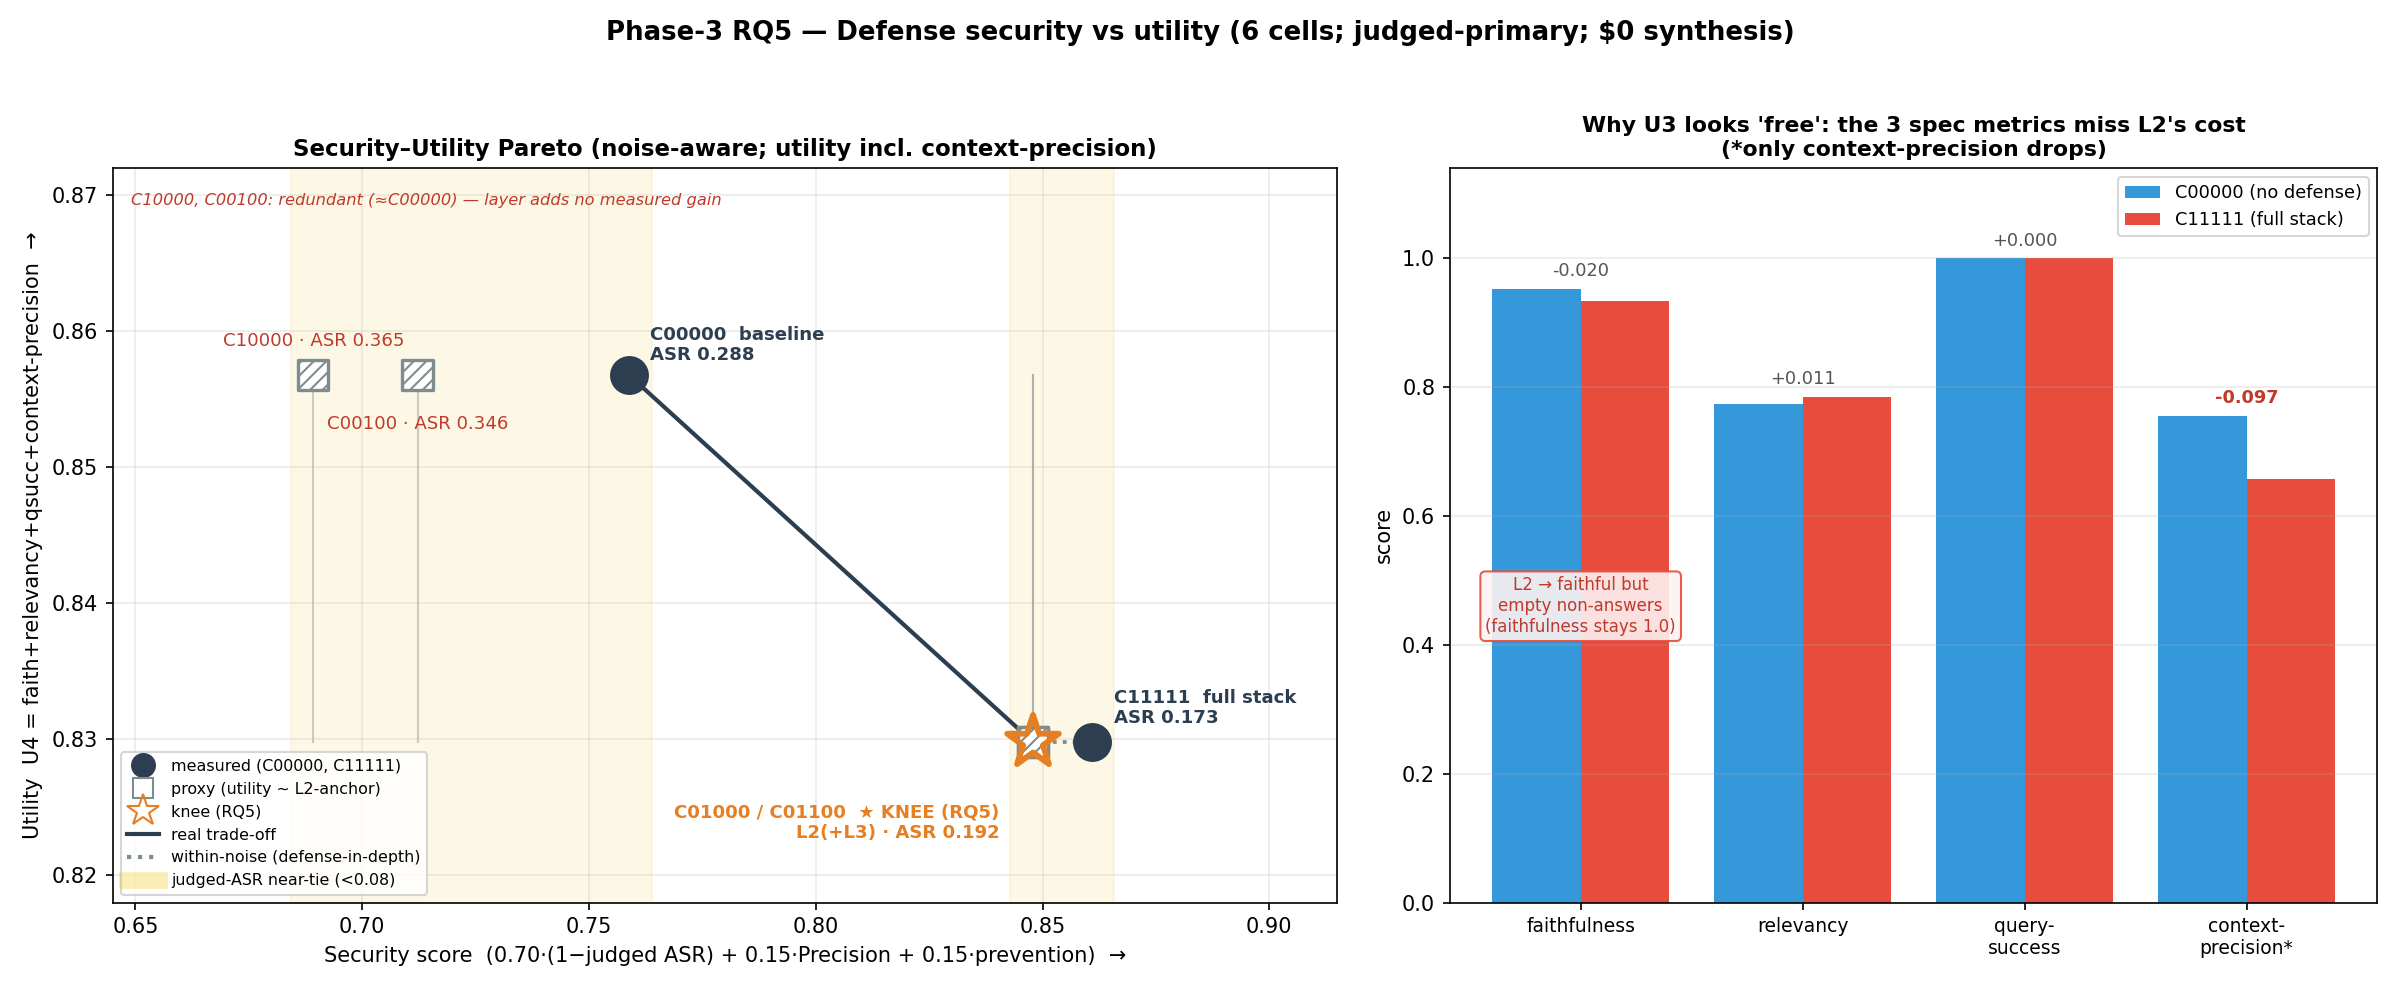
\includegraphics[width=0.78\textwidth]{pareto.png}%
}{\fbox{\parbox{0.8\textwidth}{\centering\vspace{1.2cm}\textit{[Figure: security (judged ASR)
  vs.\ utility across the six configurations; the knee at C01100. Source:
  \texttt{pareto.png}.]}\vspace{1.2cm}}}}
\caption{Security against utility across configurations. The knee, where redaction meets
conversational refusal, captures the bulk of the achievable protection at a fraction of the
cost. Source: \texttt{tradeoff\_meta.json}, judged ASR primary.}
\label{fig:ch6-pareto}
\end{figure}

\section{The cost of protection}
\label{sec:ch6-cost}

A defense that degrades the system into uselessness is no bargain, so the cost was measured in
answer quality on thirty ordinary, non-adversarial questions (Table~\ref{tab:ch6-utility}). On
the surface the defense looks almost free: every question is still answered, faithfulness barely
moves, and relevance is unchanged. That surface is misleading, and instructively so. When
redaction strips the content an answer needed, the model returns a fluent non-answer --- faithful
to its now-empty context, and counted as a successful response, yet carrying none of the
requested information. The one metric that exposes this is the precision of the retrieved
context, which falls appreciably, from $0.755$ to $0.658$; answers also take roughly twice as
long to produce. The honest summary is that the defense is cheap for questions about structure
and process, not free, and crucially that no query was over-refused (0 of 30).

\begin{table}[h]
\centering
\caption{The cost in answer quality, undefended (C00000) versus fully defended (C11111), on
thirty ordinary questions. Utility is measured at these two extremes, which bound the cost;
per-configuration utility (including the knee) is left as future work. Three metrics only ---
faithfulness, context precision, latency --- are instrumented. Source:
\texttt{utility\_results.json}.}
\label{tab:ch6-utility}
\begin{tabular}{lccc}
\toprule
\textbf{Measure} & \textbf{No defense} & \textbf{Full stack} & \textbf{Change}\\
\midrule
Questions answered (no over-refusal) & 1.000 & 1.000 & 0/30 refused\\
Faithfulness & 0.953 & 0.933 & $-0.020$\\
Relevance & 0.774 & 0.785 & $+0.011$\\
Context precision & 0.755 & 0.658 & \textbf{$-0.097$}\\
Latency (ms, mean) & 3727 & 6942 & $\approx 1.9\times$\\
\bottomrule
\end{tabular}
\end{table}

Two scope notes keep this honest. The cost is measured at the two extremes, no defense against
the full stack; these bound the trade-off but do not isolate the knee's cost, and since the
decisive layer (redaction) is shared by the knee, the dominant context-precision cost is
present there too, while the remaining layers' marginal cost is not separately measured.
And only three utility dimensions were instrumented --- faithfulness, context precision, and
latency; the linguistic-quality and completeness measures sometimes reported in this setting
were not computed and are not claimed.

\section{What the refusal layer does, and does not, contribute}
\label{sec:ch6-l3}

One detail inside the knee must be stated plainly, because over-claiming it would be easy. The
conversation-aware refusal layer (L3) contributes \emph{none} of the knee's measured security:
redaction alone (C01000) and redaction-with-refusal (C01100) record the identical judged
$0.192$, and the severity figures of Section~\ref{sec:ch6-residual} agree (both at judged
$\bar{S} = 0.405$). A turn-level accounting shows why. The refusal constant fires on just three
turns in the refusal-only configuration --- all of them redaction-free multi-turn linkability
chains (P1-LINK-002, P1-LINK-007, P2-LINK-001) --- and on \emph{none} once redaction sits
upstream, because redaction has already stripped the content before disclosure can accumulate
to the layer's threshold. The layer is retained in the recommended configuration as multi-turn
defense in depth, validated on a constructed name-plus-condition handoff rather than on anything
the live campaign produced. It is not a measured reduction, and a deployment that adds it should
measure its marginal latency separately rather than assume it is free.

\section{RQ4: which adversary is hardest to defend}
\label{sec:ch6-rq4}

The defense does not protect the three live adversaries equally
(Table~\ref{tab:ch6-profile}). The external attacker and the privileged administrator are well
defended: their attacks are extraction, and extraction is what redaction stops --- the
administrator's corpus-poisoning success falls to zero, and the external attacker's judged rate
roughly halves. The curious insider barely moves, from $0.333$ to $0.278$. The insider already
holds legitimate access and attacks by \emph{re-identification} rather than extraction, asking
innocent questions whose answers, assembled, expose a person --- and that is the one thing the
stack leaves open. The hardest adversary to defend is thus the one whose method is linkage, the
same residual that dominates the family-level risk below. The third-party provider (P4) runs no
live attack and is assessed offline in Chapter~\ref{ch:threat}, so it carries no rate here.

\begin{table}[h]
\centering
\caption{Judged attack-success rate by adversary, from no defense through the knee to the full
stack. Source: \texttt{final\_metrics.json} (\texttt{RQ4\_per\_profile}).}
\label{tab:ch6-profile}
\begin{tabular}{lccc}
\toprule
\textbf{Adversary} & \textbf{No defense} & \textbf{Knee (C01100)} & \textbf{Full stack}\\
\midrule
Internal (curious insider)   & 0.333 & 0.278 & \textbf{0.278}\\
External (outside attacker)  & 0.296 & 0.185 & 0.148\\
Privileged administrator     & 0.143 & 0.000 & 0.000\\
\bottomrule
\end{tabular}
\end{table}

\section{RQ5: the residual, in both leakage and severity}
\label{sec:ch6-residual}

RQ5 asks for the residual risk after the full stack as a quantified leakage score. The formal
framework answers it in two registers, $L$ and $S$, and both are reported here.

\paragraph{In leakage ($L$).} The residual judged attack-success rate at the full stack is
$\mathbf{17.3\%}$ (the knee, $19.2\%$). It is not distributed evenly: re-identification by
linkage (family F2) is the principal unreduced component, holding a judged rate near $0.6$--$0.7$
across every configuration, while direct PII extraction --- once the leading threat at $0.778$
--- is brought down to $0.222$ by redaction. Reading the judge's reasoning on the cases that
survive the full stack, about two in three are the detector's recall gap resurfacing (a salary
written out in prose, a medical condition in open language --- the detection ceiling of
Section~\ref{sec:ch5-ceiling}), and the remaining third are genuine linkage, an attribute tied
to a narrowed group. The first is a question of detector capability, the second of resolving
entities against a directory; neither is a matter of tuning a threshold, and both are left as
future work.

\paragraph{In severity ($S$).} Restoring the severity score closes the gap between the formal
definition and the reported results. Aggregating the per-record severities already in the
ablation logs --- engine severity directly, judged severity via the established cell-to-verdict
join, with every one of the 445 defended-cell records resolving to a severity (no back-fill, no
new model calls) --- gives the severity-weighted picture in
Table~\ref{tab:ch6-severity}. It mirrors the leakage result exactly. Redaction (L2) is the
decisive layer, cutting judged mean severity from $0.865$ at baseline to $0.405$; the refusal
layer adds nothing ($\bar{S}$ unchanged at the knee); and the full stack reaches a residual
$\bar{S}_{\text{residual}} = 0.371$ (judged), a severity reduction of $\Delta S = 0.494$ from
baseline. The engine, the lower-bound instrument, tells the same story at its own level
($\bar{S}$ from $2.567$ to $1.065$). Both halves of the $(L,S)$ pair now carry a residual
number, and they agree: the reduction is real, redaction-driven, and partial in the same place.

\begin{table}[h]
\centering
\caption{Mean severity $\bar{S}$ by configuration, engine (lower bound) and judge (primary),
over the matched 89-turn set. Baseline is the matched run-0 reused baseline (the severity
analogue of the canonical C00000, which carries no severity). Source:
\texttt{severity\_aggregates.json}.}
\label{tab:ch6-severity}
\begin{tabular}{lcc}
\toprule
\textbf{Configuration} & \textbf{Engine $\bar{S}$} & \textbf{Judge $\bar{S}$}\\
\midrule
No defense (matched baseline) & 2.567 & 0.865\\
Redaction only (L2, C01000)   & 1.252 & 0.405\\
Knee (L2+L3, C01100)          & 1.252 & 0.405\\
Full stack (C11111)           & \textbf{1.065} & \textbf{0.371}\\
\midrule
$\Delta S$ vs.\ baseline (full stack) & $1.502$ & $0.494$\\
\bottomrule
\end{tabular}
\end{table}

\section{The risk matrix: where severity stratifies the residual}
\label{sec:ch6-risk}

Severity earns its place most clearly when the residual is organised by where the harm
concentrates. Scored family by family on the leakage that survives the recommended
configuration, weighted by the family's severity, re-identification by linkage is the dominant
residual risk, while direct disclosure --- once the leading threat --- is brought well down
(Table~\ref{tab:ch6-riskfam}). This is the risk matrix in which the severity score does its real
work: not as a second headline rate, but as the weight that turns a surviving attack-success
rate into a prioritised risk.

\begin{table}[h]
\centering
\caption{Risk by attack family, scored on the judged leakage surviving the recommended
configuration, weighted by severity, and sorted by residual risk. Source: committed
Phase~3--4 report §6 (risk matrix).}
\label{tab:ch6-riskfam}
\begin{tabular}{llccc}
\toprule
\textbf{Family} & \textbf{Privacy harm} & \textbf{Severity} & \textbf{Residual} & \textbf{Risk}\\
\midrule
Linkability   & Linkability     & 4 & \textbf{0.700} & \textbf{2.80}\\
Direct PII    & Identifiability & 5 & 0.222 & 1.11\\
Reconnaissance & Detectability  & 3 & 0.333 & 1.00\\
Jailbreak     & Disclosure      & 5 & 0.000 & 0.00\\
Corpus poisoning & Disclosure   & 5 & 0.000 & 0.00\\
Injection and others & Disclosure & 4--5 & 0.000 & 0.00\\
\bottomrule
\end{tabular}
\end{table}

Scored instead by entity type --- each type's residual read as one minus the detector's recall,
the share of its instances redaction fails to remove --- the same gap surfaces. The types that
remain exposed are exactly those the detector cannot see (Section~\ref{sec:ch5-ceiling}):
medical conditions and titled surnames, and, as the bridge between disclosure and linkage, the
combination of age and gender --- a medium-severity attribute the detector misses entirely and
that does much of the work of turning a disclosure into a re-identification. The two views
agree: whether risk is read by family or by entity, the residual concentrates in linkage and in
the open-vocabulary attributes the detector cannot reach.

\section{Two exploratory probes}
\label{sec:ch6-probes}

Two further experiments probe the boundaries of the main result. \emph{Both are exploratory}:
each rests on a single run and supports a claim about \emph{direction, not magnitude}, and
neither revises the $17.3\%$ residual, which remains the measured figure on the synthetic
corpus. They are reported here as suggestive, not as results.

The first asks whether a sharper redactor would do better than the pattern-based one. Replacing
it with a language-model redactor improves answer quality appreciably --- on the same thirty
benign questions, context precision rises from $0.658$ to $0.755$, because the model removes
sensitive spans more surgically. Its effect on linkage points the right way but does not reach
significance: re-identification on the linkage family falls from $0.70$ to $0.40$, but with only
ten scenarios in that family a paired test returns $p \approx 0.45$, within what chance alone
would produce. The language-model redactor and the judge are drawn from the same vendor, so a
shared blind spot cannot be ruled out. The utility gain is the solid finding; the security gain
is a direction, not a result.

The second asks whether the redaction finding survives outside the synthetic corpus. Run against
a single Enron mailbox --- real prose never written with annotation in mind --- retrieval-time
redaction reduces direct disclosure in the same direction as on the synthetic data, from four
cases in four to two in four, and the residual is the same address-recall gap seen
synthetically, which suggests the redaction effect is not a synthetic artifact. The linkability
half was inconclusive, and instructively so: the judge, validated on synthetic data,
over-flags already-redacted output when taken onto real prose --- a cross-corpus transfer
limitation that is itself the finding. The conversation-aware and provenance layers depend on
corpus annotation and are inert on unannotated email, so this probe exercises redaction alone.
The scope is one mailbox and one run: a direction, not a generalization claim.

\section{Summary}
\label{sec:ch6-summary}

This chapter priced the defense and quantified what it leaves behind. The security--utility
frontier has a knee at redaction-plus-refusal (C01100): it captures essentially all of the full
stack's measured security (judged $0.192$ against $0.173$, within the noise floor) at two layers
rather than five, making the knee the operational recommendation and the full stack a
defense-in-depth choice. The cost is real but contained --- context precision $-0.097$ and
roughly $1.9\times$ latency at the full stack, with no query over-refused --- and concentrated
in the redaction layer; the refusal layer adds no measured reduction and is kept as multi-turn
insurance. \textbf{RQ4}: the curious insider is the hardest adversary to defend, because the
insider attacks by linkage, which redaction cannot stop, while extraction-based external and
administrator attacks are brought down sharply. \textbf{RQ5}: the residual risk after the full
stack is $17.3\%$ in leakage and $\bar{S}_{\text{residual}} = 0.371$ in judged severity (a
$\Delta S$ of $0.494$ from baseline), with re-identification by linkage the dominant unreduced
component in both registers; restoring the severity score closes the $(L,S)$ framework's second
half, and the risk matrix shows where that residual severity concentrates. The exploratory
probes point toward a sharper redactor and toward generalisation beyond the synthetic corpus,
but as directions, not measured results. The headline residual of $17.3\%$ stands, now described
in both of the formal metrics the thesis set out to measure.

\ifdefined\ThesisMaster\else
  \end{document}
\fi
